\chapter{Grundlagen}


\section{Wasserstoff-Elektrolyse}
Unter Wasserstoff-Elektrolyse versteht man grundlegend die Funktion Wasser in seine Bestandteile Wasserstoff und Sauerstoff zu spalten. Die verbreitetste Variante ist die alkalische Elektrolyse, welche bereits im großen Maßstab eingesetzt wird. Unter anderem in einer zwei Gigawatt Anlage in Saudi-Arabien \cite{2GWely} . Des weiteren wird viel Potential in der Weiterentwicklung der PEM Elektrolyse gesetzt, da diese durch einen simpleren Aufbau und höhere Stromdichten bessere Skalierbarkeit bieten kann. Außerdem wird die Hochtemperatur Elektrolyse verwendet, wenn sich die Nutzung von Prozess technischer Abwärme anbietet, wodurch der Gesamtwirkungsgrad steigt \cite{Elektrolyse}.  

\section{Stromrichter}
\subsection{Gleichrichter}
Ein Gleichrichter wird verwendet, um aus einer Wechselspannung eine Gleichspannung zu erzeugen. Die einfachste Form ist der Diodengleichrichter, dieser kann für einphasige Wechselspannung durch eine einzelne Diode realisiert werden. Jedoch würde so nur die halbe Periode des Sinus am Ausgang zur Verfügung stehen, da die Diode nur während der positiven Halbwelle Leitet. Dies lässt sich durch die Ergänzung zum Brückengleichrichter mit vier und für dreiphasige Anwendungen mit sechs Dioden ausgestattet ist.\\
Anhand des Diodengleichrichters wird schnell klar, dass eine solche Schaltung nur bedingt für einen gewünschten Stromverlauf sorgt. In Abbildung \ref{B6DiodRect} sind Netzspannung und Strom dargestellt, der Stromverlauf zeigt Starke Sprünge und der gewünschte Sinusförmige Verlauf ist nur schwer erkennbar. Außerdem lässt sich mit dieser Schaltung die Ausgangsspannung sowie der Strom nicht variieren.
\begin{figure}
	\centering
	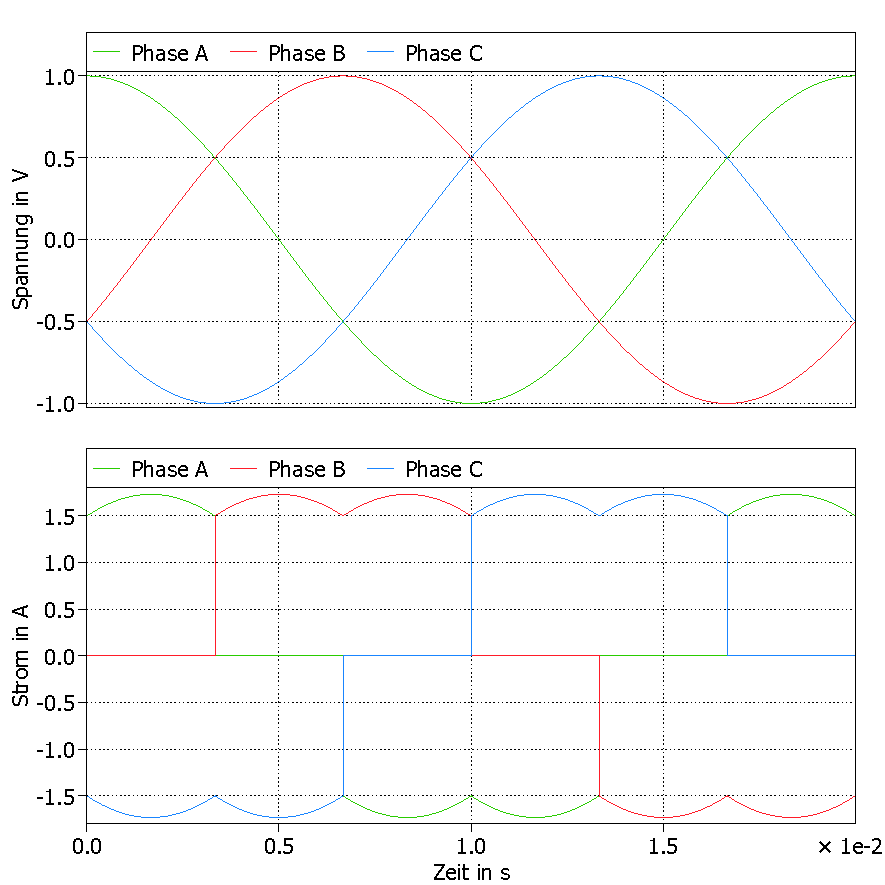
\includegraphics[width=0.7\linewidth]{content/Grafiken/B6-Diodengleichrichter-Eingangsverlauf}
	\caption{Strom und Spannungsverlauf am B6 Diodengleichrichter}
	\label{B6DiodRect}
\end{figure}



ungesteuerte Topologien

Netz gesteuerte Topologien

\subsection{DC-DC Wandler}
Der Hoch- und Tiefsetzsteller sind essenzielle Topologien und bestehen im wesentlichen aus einer Diode, einem Schalter und einer Induktivität. 
	
\subsection{Power Factor Correction}
	Die \gls{PFC} ist eine nötige Maßnahme um den Blindleistungsanteil im Netz zu reduzieren 
	The front-end circuit concept of the H3R system was first introduced in late 90s by Jantsch and Verhoeve,
	
	
\section{IAF Rectifier}
Der \gls{IAF} Gleichrichter wurde erstmals vorgestellt in \cite{IAFfirst} im Jahr 1997 . Dieser besteht für den Hauptleistungspfad aus einem Diodengleichrichter, um sinusförmige Ströme in allen drei Phasen einzuprägen wird dieser durch ein Netzwerk aus bidirektional Sperrenden Leistungshalbleitern ergänzt, welche einen Strom in den Gleichrichter einprägen. Durch die Integration des Filters in den Leistungspfad, kann die Kompensation effizienter funktionieren. Aufgrund des ungesteuerten Diodengleichrichters wird jedoch eine anschließende Spannungsregelung durch einen Tiefsetzsteller benötigt.

\section{1/3 PWM PFC Rectifier}
Bei dieser Topologie handelt es sich um eine gängige Schaltung, welche durch ein neuartiges Modulationsverfahren unter Verwendung von Induktivitäten auf der Netzseite eine Reduzierung der Schaltverluste bewirkt und Blindleistung ermöglicht. Das Verfahren wurde ausführlich von Menzi, Bortis und Kolar beschrieben \cite{13PWMPFC}.



\section{Leistungshalbleiter}

\section{Induktivitäten}

\section{Simulationssoftware}
Zur Bewertung und Betrachtung der Umsetzbarkeit, der Topologien ist es nötig diese in einer Umfassenden Simulation zu betrachten. Dies ermöglicht es die Funktionalität und den Einfluss der Parameter im direkten Zusammenspiel zu untersuchen. Insbesondere das Verhalten für Systemdienstleistungen, wie Phasenverschiebung und die dadurch beeinflusste Verteilung der Verlustleistungen sollen als Entscheidungsgrundlage dienen. 

	\subsection{PLECS}